\documentclass[10 pt,usenames,dvipsnames, oneside]{article}

\makeatletter
\newcommand{\dontusepackage}[2][]{%
  \@namedef{ver@#2.sty}{9999/12/31}%
  \@namedef{opt@#2.sty}{#1}}
\makeatother
\dontusepackage{tabu}
\usepackage{../../../modelo-ensino-medio}

\usepackage{tabu-2019}

\begin{document}

\begin{center}
  \begin{minipage}[l]{3cm}
\includegraphics[width=2cm]{logo}    
\end{minipage}\hfill
\begin{minipage}[r]{.8\textwidth}
 {\Large \scshape Atividade: A água continua subindo}  
\end{minipage}
\end{center}
\vspace{.2cm}

\ifdefined\prof
\begin{objetivos}
\item \textbf{LAF2} Compreender a taxa de variação como uma medida de covariação entre grandezas e utilizá-la para interpretar situações reais.
\end{objetivos}

\begin{goals}
\begin{enumerate}

\item [OE1] Registrar em palavras diversas situações que são descritas por funções crescentes, especificando mudanças de comportamento. 

\end{enumerate}

\tcblower
 
\begin{itemize}
\item Considere realizar essa atividade em grupo, principalmente em turmas maiores. Essa pode ser uma estratégia interessante para dar oportunidade para que os estudantes, em grupos, exponham suas impressões e argumentos.
\item Após os estudantes realizarem as análises, discuta com eles sobre a necessidade de se ter uma maneira sistemática de diferenciar as diversas maneiras que se pode ter um gráfico crescente.
\item Estimule-os a pensar em outras situações em que há variações similares ou situações análogas em que haja decrescimento.
\item Certifique-se que todos os estudantes compreendem o significado de "vazão constante", isto é, que o volume de água por unidade de tempo que entra em cada um dos recipientes é constante.
\item Aqui a palavra uniformemente deve ser interpretada a partir do senso comum: aquilo
que não tem variação ou mudança. Mais adiante será apresentada uma definição
precisa para o que devemos entender como crescimento/decrescimento uniforme.
\end{itemize}

\end{goals}

\bigskip
\begin{center}
{\large \scshape Atividade}
\end{center}
\fi

\textbf{Parte I} Suponha que os diversos reservatórios abaixo têm a mesma capacidade, a mesma altura e que em cada um deles a água entra a uma vazão constante. Analisando a forma de cada um dos reservatórios, descreva de que maneira a altura varia em função do tempo no início, meio e fim do processo. Use, quando necessário, as palavras \textbf{lentamente}, \textbf{rapidamente} e \textbf{uniformemente}. (Gravina, 1992, pp. 33-38)

\setlength\abovetabulinesep{2mm}
\begin{longtabu} to \textwidth{|c|@{\hspace{0.8\textwidth}}|}
\endfirsthead
\hline
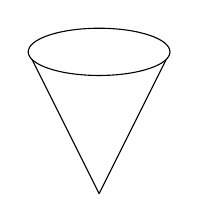
\begin{tikzpicture}[scale=.3]

\draw (-3,0) -- (0,-6);
\draw (3,0) -- (0,-6);
\draw [fill=white] (0,0) ellipse [x radius=3,y radius=1];

\end{tikzpicture}\\
\hline
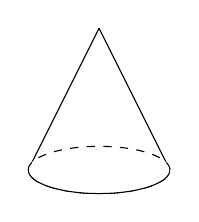
\begin{tikzpicture}[scale=.3]

\draw (-3,0) -- (0,6);
\draw (3,0) -- (0,6);

\draw [fill=white, dashed] (0,0) ellipse [x radius=3,y radius=1];
\clip (-3,0) rectangle (3,-1);
\draw [fill=white] (0,0) ellipse [x radius=3,y radius=1];

\end{tikzpicture}\\
\hline
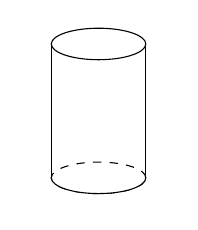
\begin{tikzpicture}[scale=.3]

\draw (-2,0) -- (-2,5+2/3);
\draw (2,0) -- (2,5+2/3);

\draw [fill=white] (0,5+2/3) ellipse [x radius=2,y radius=2/3];

\draw [fill=white, dashed] (0,0) ellipse [x radius=2,y radius=2/3];
\clip (-3,0) rectangle (3,-1);
\draw [fill=white] (0,0) ellipse [x radius=2,y radius=2/3];


\end{tikzpicture}\\
\hline
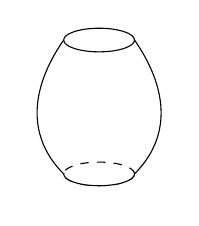
\begin{tikzpicture}[scale=.3]

\draw (-1.5,0) .. controls (-3,1.5) and (-3,3.5) .. (-1.5,5+2/3);
\draw (1.5,0) .. controls (3,1.5) and (3,3.5) .. (1.5,5+2/3);

\draw [fill=white] (0,5+2/3) ellipse [x radius=1.5,y radius=2/3*3/4];

\draw [fill=white, dashed] (0,0) ellipse [x radius=1.5,y radius=2/3*3/4];
\clip (-3,0) rectangle (3,-1);
\draw [fill=white] (0,0) ellipse [x radius=1.5,y radius=2/3*3/4];


\end{tikzpicture}\\
\hline
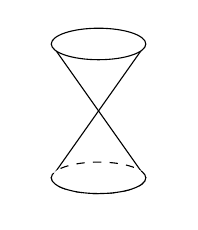
\begin{tikzpicture}[scale=.3]

\draw (-2,0) -- (2,5+2/3);
\draw (2,0) -- (-2,5+2/3);

\draw [fill=white] (0,5+2/3) ellipse [x radius=2,y radius=2/3];

\draw [fill=white, dashed] (0,0) ellipse [x radius=2,y radius=2/3];
\clip (-3,0) rectangle (3,-1);
\draw [fill=white] (0,0) ellipse [x radius=2,y radius=2/3];


\end{tikzpicture}\\
\hline
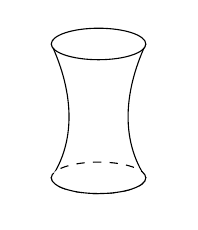
\begin{tikzpicture}[scale=.3]

\draw (-2,0) .. controls (-1,1.5) and (-1,3.5) .. (-2,5+2/3);
\draw (2,0) .. controls (1,1.5) and (1,3.5) .. (2,5+2/3);

\draw [fill=white] (0,5+2/3) ellipse [x radius=2,y radius=2/3];

\draw [fill=white, dashed] (0,0) ellipse [x radius=2,y radius=2/3];
\clip (-3,0) rectangle (3,-1);
\draw [fill=white] (0,0) ellipse [x radius=2,y radius=2/3];


\end{tikzpicture}\\
\hline
\end{longtabu}

\ifx\prof\undefined
\clearpage
\fi

\textbf{Parte II} Relacione a forma do pote com o gráfico da variação da altura em função do tempo de cada um deles.

\setlength{\columnsep}{0pt}

\begin{multicols}{3}

\begin{enumerate}
\setlength{\itemsep}{0pt}
\setlength{\parskip}{0pt}

\item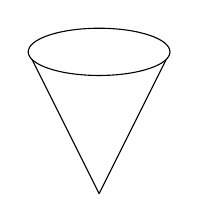
\begin{tikzpicture}[scale=.3,baseline=(current bounding box.north)]

\draw (-3,0) -- (0,-6);
\draw (3,0) -- (0,-6);
\draw [fill=white] (0,0) ellipse [x radius=3,y radius=1];

\end{tikzpicture}

\item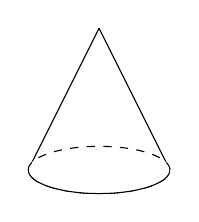
\begin{tikzpicture}[scale=.3,baseline=(current bounding box.north)]

\draw (-3,0) -- (0,6);
\draw (3,0) -- (0,6);

\draw [fill=white, dashed] (0,0) ellipse [x radius=3,y radius=1];
\clip (-3,0) rectangle (3,-1);
\draw [fill=white] (0,0) ellipse [x radius=3,y radius=1];

\end{tikzpicture}

\item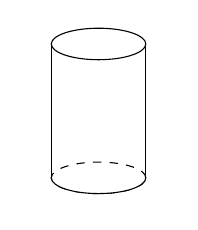
\begin{tikzpicture}[scale=.3,baseline=(current bounding box.north)]

\draw (-2,0) -- (-2,5+2/3);
\draw (2,0) -- (2,5+2/3);

\draw [fill=white] (0,5+2/3) ellipse [x radius=2,y radius=2/3];

\draw [fill=white, dashed] (0,0) ellipse [x radius=2,y radius=2/3];
\clip (-3,0) rectangle (3,-1);
\draw [fill=white] (0,0) ellipse [x radius=2,y radius=2/3];


\end{tikzpicture}

\item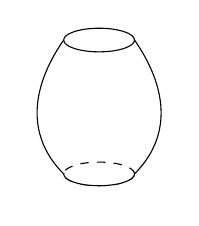
\begin{tikzpicture}[scale=.3,baseline=(current bounding box.north)]

\draw (-1.5,0) .. controls (-3,1.5) and (-3,3.5) .. (-1.5,5+2/3);
\draw (1.5,0) .. controls (3,1.5) and (3,3.5) .. (1.5,5+2/3);

\draw [fill=white] (0,5+2/3) ellipse [x radius=1.5,y radius=2/3*3/4];

\draw [fill=white, dashed] (0,0) ellipse [x radius=1.5,y radius=2/3*3/4];
\clip (-3,0) rectangle (3,-1);
\draw [fill=white] (0,0) ellipse [x radius=1.5,y radius=2/3*3/4];


\end{tikzpicture}

\item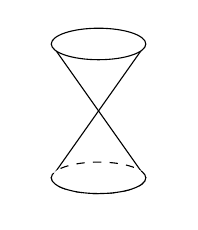
\begin{tikzpicture}[scale=.3,baseline=(current bounding box.north)]

\draw (-2,0) -- (2,5+2/3);
\draw (2,0) -- (-2,5+2/3);

\draw [fill=white] (0,5+2/3) ellipse [x radius=2,y radius=2/3];

\draw [fill=white, dashed] (0,0) ellipse [x radius=2,y radius=2/3];
\clip (-3,0) rectangle (3,-1);
\draw [fill=white] (0,0) ellipse [x radius=2,y radius=2/3];


\end{tikzpicture}

\item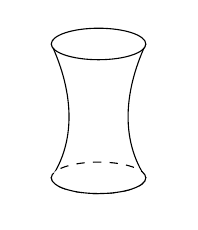
\begin{tikzpicture}[scale=.3,baseline=(current bounding box.north)]

\draw (-2,0) .. controls (-1,1.5) and (-1,3.5) .. (-2,5+2/3);
\draw (2,0) .. controls (1,1.5) and (1,3.5) .. (2,5+2/3);

\draw [fill=white] (0,5+2/3) ellipse [x radius=2,y radius=2/3];

\draw [fill=white, dashed] (0,0) ellipse [x radius=2,y radius=2/3];
\clip (-3,0) rectangle (3,-1);
\draw [fill=white] (0,0) ellipse [x radius=2,y radius=2/3];


\end{tikzpicture}
\end{enumerate}
\end{multicols}

% \begin{figure}[H]
% \centering
% \includegraphics[width=350bp]{taxa-ativ-2-7}

% \end{figure}

\begin{multicols}{3}
\begin{enumerate}[label=(\Roman*)]
\item \begin{tikzpicture}[scale=.4,baseline=(current bounding box.north), every node/.style={scale=.8}]


\draw [->] (0,0) -- (5,0) node [below] {T};
\draw [->] (0,0) -- (0,5) node [left] {A};

\clip (0,0) rectangle (4,4);
\draw [dashed] (4,0) -- (4,4) -- (0,4);

\draw [thick] (0,0) .. controls (3,2) and (2,3) ..  (4,4);

\end{tikzpicture}

\item\begin{tikzpicture}[scale=.4,baseline=(current bounding box.north), every node/.style={scale=.8}]


\draw [->] (0,0) -- (5,0) node [below] {T};
\draw [->] (0,0) -- (0,5) node [left] {A};

\clip (0,0) rectangle (4,4);
\draw [dashed] (4,0) -- (4,4) -- (0,4);

\draw [thick] (4,0) circle (4);

\end{tikzpicture}

\item\begin{tikzpicture}[scale=.4,baseline=(current bounding box.north), every node/.style={scale=.8}]


\draw [->] (0,0) -- (5,0) node [below] {T};
\draw [->] (0,0) -- (0,5) node [left] {A};

\clip (0,0) rectangle (4,4);
\draw [dashed] (4,0) -- (4,4) -- (0,4);

\draw [thick] (0,0) .. controls (1,3) and (3,1) ..  (4,4);

\end{tikzpicture}

\item\begin{tikzpicture}[scale=.4,baseline=(current bounding box.north), every node/.style={scale=.8}]


\draw [->] (0,0) -- (5,0) node [below] {T};
\draw [->] (0,0) -- (0,5) node [left] {A};

\clip (0,0) rectangle (4,4);
\draw [dashed] (4,0) -- (4,4) -- (0,4);

\draw [thick] (0,0) .. controls (3,1) and (1,3) ..  (4,4);

\end{tikzpicture}

\item\begin{tikzpicture}[scale=.4,baseline=(current bounding box.north), every node/.style={scale=.8}]


\draw [->] (0,0) -- (5,0) node [below] {T};
\draw [->] (0,0) -- (0,5) node [left] {A};

\clip (0,0) rectangle (4,4);
\draw [dashed] (4,0) -- (4,4) -- (0,4);

\draw [thick] (0,4) circle (4);

\end{tikzpicture}

\item\begin{tikzpicture}[scale=.4,baseline=(current bounding box.north), every node/.style={scale=.8}]


\draw [->] (0,0) -- (5,0) node [below] {T};
\draw [->] (0,0) -- (0,5) node [left] {A};

\draw [dashed] (4,0) -- (4,4) -- (0,4);

\draw [thick] (0,0) -- (4,4);

\end{tikzpicture}

\end{enumerate}
\end{multicols}

\ifdefined\prof

\begin{solucao}

Admitinho que a água entra a uma taxa constante em cada um dos recipientes, podemos descrever a maneira como a altura da coluna de água varia com o tempo da seguinte forma:

\setlength\abovetabulinesep{2mm}
\begin{longtabu}{|>{\centering\vspace{.5em}}m{.15\linewidth}<{\vspace{-.5em}}|>{\centering}m{.6\linewidth}|>{\centering}m{.1\linewidth}|}
\endfirsthead
\hline
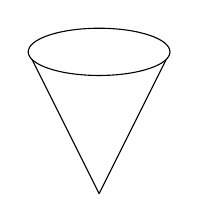
\begin{tikzpicture}[scale=.3]
\vspace{1em}
\draw (-3,0) -- (0,-6);
\draw (3,0) -- (0,-6);
\draw [fill=white] (0,0) ellipse [x radius=3,y radius=1];

\end{tikzpicture}
\vspace{1em} & No início a coluna de água subirá rapidamente, no meio estará subindo mais lentamente e na parte final mais lentamente ainda. & (II) \\
\hline
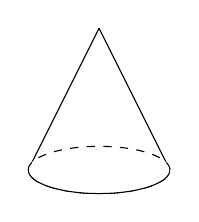
\begin{tikzpicture}[scale=.3]

\draw (-3,0) -- (0,6);
\draw (3,0) -- (0,6);

\draw [fill=white, dashed] (0,0) ellipse [x radius=3,y radius=1];
\clip (-3,0) rectangle (3,-1);
\draw [fill=white] (0,0) ellipse [x radius=3,y radius=1];

\end{tikzpicture}

& No início a coluna de água subirá lentamente, no meio estará subindo mais rapidamente e na parte final mais rapidamente ainda. & (V)\\
\hline
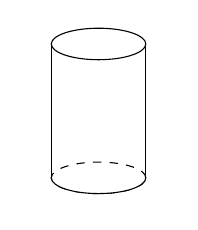
\begin{tikzpicture}[scale=.3]

\draw (-2,0) -- (-2,5+2/3);
\draw (2,0) -- (2,5+2/3);

\draw [fill=white] (0,5+2/3) ellipse [x radius=2,y radius=2/3];

\draw [fill=white, dashed] (0,0) ellipse [x radius=2,y radius=2/3];
\clip (-3,0) rectangle (3,-1);
\draw [fill=white] (0,0) ellipse [x radius=2,y radius=2/3];


\end{tikzpicture}

& A altura da água subirá de maneira uniforme, com velocidade constante & (VI)\\
\hline
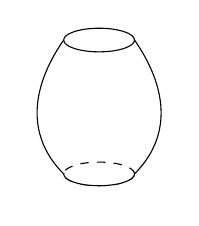
\begin{tikzpicture}[scale=.3]

\draw (-1.5,0) .. controls (-3,1.5) and (-3,3.5) .. (-1.5,5+2/3);
\draw (1.5,0) .. controls (3,1.5) and (3,3.5) .. (1.5,5+2/3);

\draw [fill=white] (0,5+2/3) ellipse [x radius=1.5,y radius=2/3*3/4];

\draw [fill=white, dashed] (0,0) ellipse [x radius=1.5,y radius=2/3*3/4];
\clip (-3,0) rectangle (3,-1);
\draw [fill=white] (0,0) ellipse [x radius=1.5,y radius=2/3*3/4];


\end{tikzpicture}

& No início a altura de coluna subirá mais rapidamente, ficando cada vez mais lenta até chgar à metade do recipiente. Daí em diante, de maneira simétrica, voltará a acelerar. & (III) \\
\hline
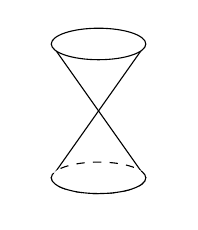
\begin{tikzpicture}[scale=.3]

\draw (-2,0) -- (2,5+2/3);
\draw (2,0) -- (-2,5+2/3);

\draw [fill=white] (0,5+2/3) ellipse [x radius=2,y radius=2/3];

\draw [fill=white, dashed] (0,0) ellipse [x radius=2,y radius=2/3];
\clip (-3,0) rectangle (3,-1);
\draw [fill=white] (0,0) ellipse [x radius=2,y radius=2/3];


\end{tikzpicture}

& No início a altura da coluna de água subirá lentamente, ficando cada vez mais rápida até chegar à metade do recipiente. Daí em diante, de maneira simétrica, voltará a descelerar. & (IV)\\
\hline
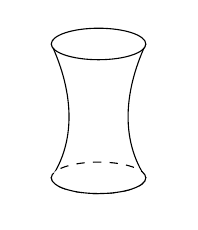
\begin{tikzpicture}[scale=.3]

\draw (-2,0) .. controls (-1,1.5) and (-1,3.5) .. (-2,5+2/3);
\draw (2,0) .. controls (1,1.5) and (1,3.5) .. (2,5+2/3);

\draw [fill=white] (0,5+2/3) ellipse [x radius=2,y radius=2/3];

\draw [fill=white, dashed] (0,0) ellipse [x radius=2,y radius=2/3];
\clip (-3,0) rectangle (3,-1);
\draw [fill=white] (0,0) ellipse [x radius=2,y radius=2/3];


\end{tikzpicture}

& Comportamento similar ao anterior, contudo, as diferenças de velocidade não são tão perceptíveis. Pode funcionar como um "meio termo"{} entre o anterior e o cilíndro. & (I)\\
\hline
\end{longtabu}
\end{solucao}
\fi

\end{document}